\section{\Tool design}
\label{sec:design}
\Tool is composed of a series of analysis routines, each designed to 
identify whether a given loop belongs to one specific type of root causes,
as we will present below. 

As briefly mentioned in Section \ref{sec:intro}, the design of these analysis routines follows the following principles.
\begin{itemize}
\item Providing diagnosis information, not detecting bugs. \Tool will be  
used together with other performance diagnosis tools \cite{SongOOPSLA2014}
and focus on a small
number of loops that are most correlated with a specific performance symptom,
instead of being applied to the whole program. Therefore, we will have different
design trade-offs in terms of coverage and accuracy, comparing with 
bug detection tools.

\item Static-dynamic hybrid analysis. As we will see, static analysis alone
will not be able to provide all the needed information for performance
diagnosis; dynamic analysis alone will incur too much unnecessary overhead.
Therefore, we will use static-dynamic hybrid approach throughout our design.

\item Using sampling to decrease run-time overhead. Loop-related 
performance problems have the unique nature of repetitiveness, which make 
them a natural fit for random sampling. Therefore, we will design different
sampling schemes for different analysis routines.
\end{itemize}

\subsection{Resultless Checker}
\label{sec:workless}

Our resultless checker includes two parts. First, we use static analysis
to figure out which are the side-effect instructions in a loop and hence
decide whether a loop belongs to 0*, 0*1?, [0$|$1]*, or 1*. Second, for
0*1? and [0$|$1]* loops, we use
dynamic analysis to figure out what portion of loop iterations are
resultless at run time, which will help decide whether the loop is indeed
inefficient.

%\begin{figure}[ht]
%\center
%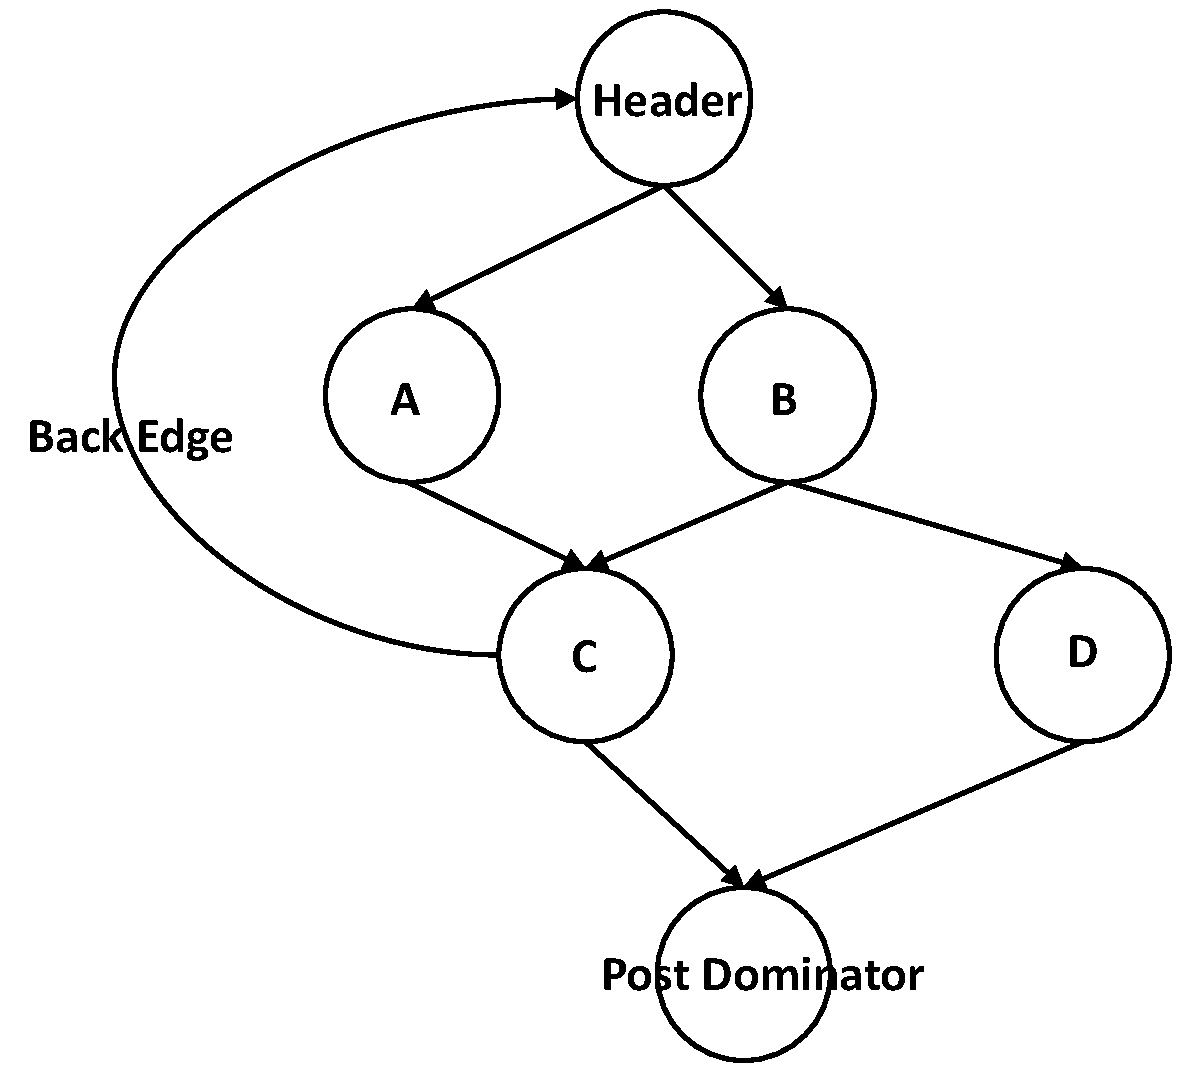
\includegraphics[width=0.7\linewidth]{figures/workless.pdf}
%\caption{Examples for different types of basic blocks inside a loop}
%\label{fig:block_type}
%\end{figure}

\subsubsection{Static Analysis}
\label{sec:s_workless}

We consider side-effect instructions as those instructions that write to
variables defined outside the loop. The analysis to identify side-effect
instructions is straightforward. We consider all functions that are called
by a loop directly or indirectly --- a function $F$ that updates variables
defined outside $F$ makes the corresponding call statement in $F$'s
caller a side-effect instruction.
We consider all library functions or function calls through function pointers 
as functions that have side effects, 
unless the library functions are specially marked by us in a white list.

After identifying side-effect instructions, it is straight-forward to
categorize loops into the four types discussed above.
Loop 0* contains no side-effect instructions. 
Loop 1* contains at least one side-effect instruction along every path that
starts from the loop header and ends at the loop header.
The remaining cases are either 
0*1? or [0$|$1]*. 
Differentiating these two cases is also straight-forward.
In short, when the basic block that contains side-effect instructions
is part of the natural loop, the case
belongs to [0$|$1]*; instead, if the side-effect basic block is post-dominated
by one of the loop-exit blocks and is dominated by the loop header, yet is
not part of the natural loop, the case belongs to 0*1?.

Finally, since the 1* pattern contains the least amount of information
about computation \textit{inefficiency}, \Tool will not report a loop's
root-cause type as 1*, if more informative root-cause type is identified 
for this loop (e.g., cross-iteration or cross-loop redundancy).

%TODO Shan will rewrite the next two paragraphs
\subsubsection{Dynamic Monitoring}
\label{sec:d_workless}

Except for 0*, none of the other three type of loops are inefficient for sure.
We need dynamic analysis to figure out what portion of loop iterations are
resultless at run time, which will help decide whether the loop is indeed
the root cause of a user-perceived performance problem and worth fixing.

For a 0*1? loop, since it only generates results in the last iteration, we 
only need to know the total number of iterations (or the average total number 
of iterations when the loop has multiple instances) to figure out the 
\textit{resultless rate} of the loop. The implementation is straightforward
--- we initialize a local counter to be 0 in the pre-header of the loop; we 
increase the counter by 1 in the loop header to count the number of 
iterations; we dump that counter to log when the loop exits.

For [0$|$1]*, we need to count not only the total number of iterations, but
also the exact number of iterations that execute side-effect instructions
at run time. 
To do that, our instrumentation uses a local boolean variable 
\texttt{HasResult} to represent whether one iteration have side effect or not. 
\texttt{HasResult} is set to \texttt{False} in the loop header, and set to
\texttt{True} after each side-effect instruction. It will be used to help
count the number of side-effect iterations. For performance concerns,
before instrumenting side-effect blocks, we check whether there are 
post-domination relation between each pair of side-effect blocks. 
If both block A and block B are side-effect blocks and block A post-dominates 
block B, we only instrument block A to update \texttt{HasResult}. 

We could speed up the above counting using sampling. However, since the 
run-time overhead of the above counting is low, as shown in Section 
\ref{sec:experiment}, our current prototype of \Tool does 
not use sampling for this part of run-time analysis.

%\subsubsection{Sampling}
%We calculate the average iteration number 
%and the ratio of working iteration based on a separated 
%process from on-line branch sampling discussed in~\cite{SongOOPSLA2014}.
%We need to instrument the buggy program and re-execute it by using bug-triggering input. 
%In the future, we could design an algorithm to calculate the two resultless metrics 
%based on branch sampling reports to get rid of the extra instrumentation and the extra bad run.   

\subsubsection{Limitations}
\label{sec:l_workless}
The technique designed in this section has the following limitations.
First, when callee may have side effect, we will consider it will have side effect in the caller side, 
and do not consider the real execution inside callee. This could bring false negatives, 
because we could miss resultless cases, 
where side effect instructions inside callee do not execute. 
Experiments results in Section~\ref{sec:experiment} show that this is not a big issue, 
since we do not miss any resultless bugs.  

Second, our dynamic instrumentation does not consider concurrent execution of the monitored loop, 
because most of buggy loops we study only execute in one single thread. 
When the monitored loop is executed in multi-thread, like loop marked with omp pragma, we need to synchronize updates to global variables. 
